%& -shell-escape 
% $Header: /cvsroot/latex-beamer/latex-beamer/solutions/conference-talks/conference-ornate-20min.en.tex,v 1.7 2007/01/28 20:48:23 tantau Exp $
\documentclass[ignorenonframetext]{beamer}

\mode<article>{\usepackage{fullpage}}
\mode<presentation>
{
  \usetheme{Marburg}   
  \usecolortheme{default}
}
\usepackage[dutch]{babel}
\usepackage[latin1]{inputenc}
\usepackage{times}
%\usepackage[round]{natbib}
\usepackage[T1]{fontenc}
\usepackage{tikz}
\usetikzlibrary{arrows, shapes} 
\usetikzlibrary{backgrounds}
\usetikzlibrary{fit}
\tikzstyle{every picture}+=[remember picture]
\everymath{\displaystyle}
\usepackage{relsize}

\pgfdeclarelayer{background}
\pgfdeclarelayer{foreground}
\pgfsetlayers{background,main,foreground}
\usepackage{animate}
\usepackage{extarrows}
\usepackage{microtype, graphicx, booktabs,amssymb, relsize, bm, booktabs, amsmath, subfigure,
calc, amsthm, marvosym, dcolumn}
\usepackage{pgfplots}
\setbeamertemplate{navigation symbols}{}  

\title[Spatial Stochastic Frontiers]
{On spatial dependence in stochastic frontier models with an application to European regional economic performance}

\author[Thomas de Graaff] % (optional, use only with lots of authors)
{Thomas~de~Graaff}

\date[GfR-Conference] % (optional, should be abbreviation of conference name)
{GfR-Conference, Marburg, 26 juni 2014}

\institute[] % (optional, but mostly needed)
{
  Department of Spatial Economics,  Vrije Universiteit Amsterdam\\
  \url{https://github.com/thdegraaff}
}

\begin{document}
\begin{frame}
  \titlepage
\end{frame}

\section{Why bother?}

\subsection{Background}

\begin{frame}
\frametitle{GDP per capita across Europe in 2007---EU27 = 100 (source: cambridge econometrics database}
\begin{figure}[h]
	\center
	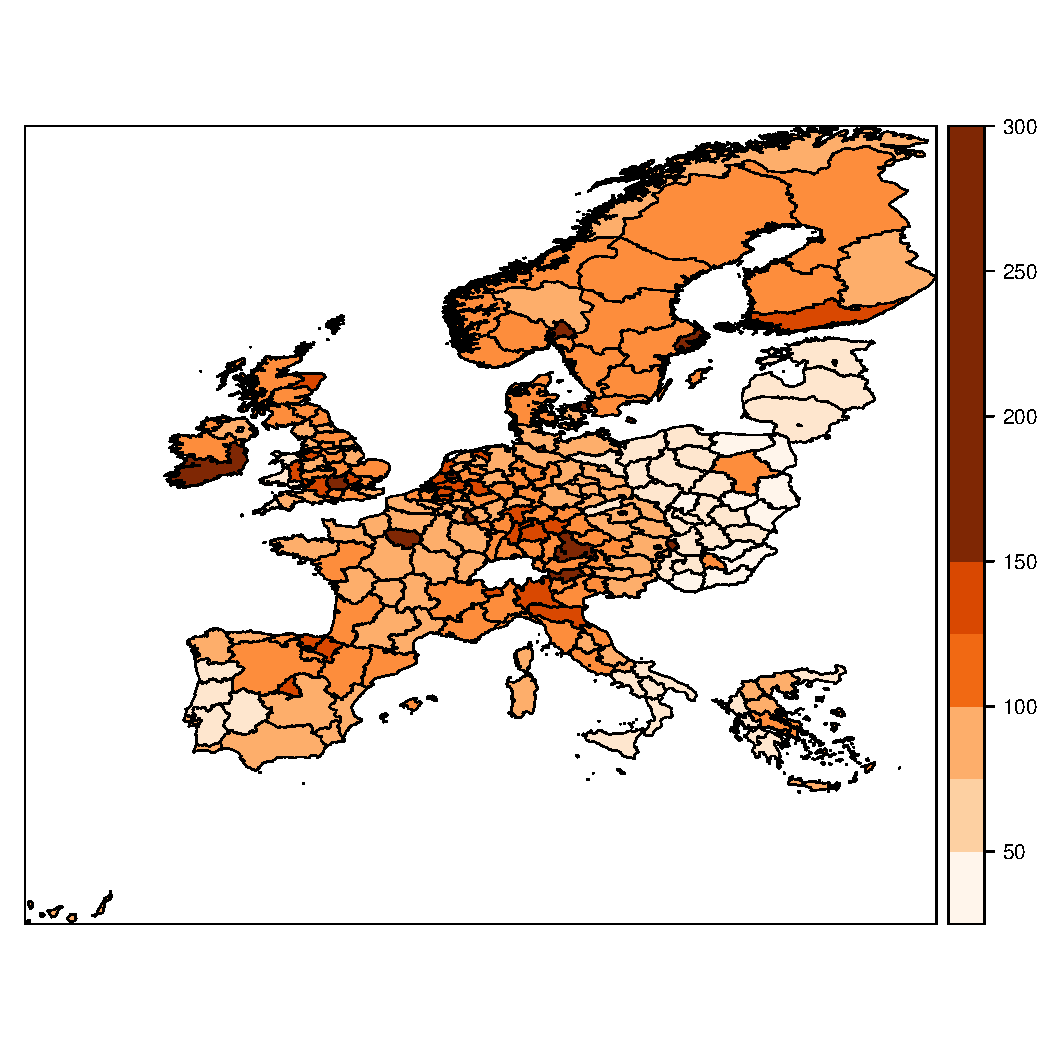
\includegraphics[width=0.8\textwidth]{gdppc}
\end{figure}
\end{frame}

\begin{frame}{Background \& research question}
\begin{block}{How to benchmark the economic performance of European regions in the presence of networks}
\begin{itemize}
	\item Data Envelopment Analysis vs Stochastic Frontier Analysis	
	\item Absolute efficiency: the efficiency of the use of input factors vs relative efficiency: accessibility to knowledge/technology
	\item Relevant for policy 
	\begin{itemize}
		\item Place-based policies versus place-neutral policies (Barca, 2011)
		\item Determinants of economic performance might vary over space (Thissen et al., 2013)
	\end{itemize}
\end{itemize}
\end{block}
\end{frame}

\subsection{Literature}

\begin{frame}{Related literature}
	\begin{itemize}
		\item Starting point: Weinstein (Technometrics, 1964)
		\begin{itemize}
			\item Econometric literature: Aigner et al. (1977); Meeusen \& van den Broeck (1977). 
			\item Statistical literature: Azzalini (1985); Azzalini \& Capitanio (1999); Dominguez-Molina et al. (2003)
		\end{itemize}
		\pause
		\item Regional stochastic frontiers: Puig-Junoy (2001); Alvarez (2007)
		\pause
		\item Recent literature concerning spatial stochastic frontiers: 
	\begin{itemize}
		\item Parametric approach: Pavlyuk (2010); Barrios \& Lavado (2010)
		\item Bayesian approach: Schmidt et al. (2009); Areal et al. (2010)
	\end{itemize}
	\end{itemize}
\end{frame} 

\section{Benchmarking regions}

\subsection{Frontiers in production}

\begin{frame}{Production Isoquant}
\tikzstyle{background}=[circle, fill=gray!30,inner sep=0.5cm]
\begin{center}
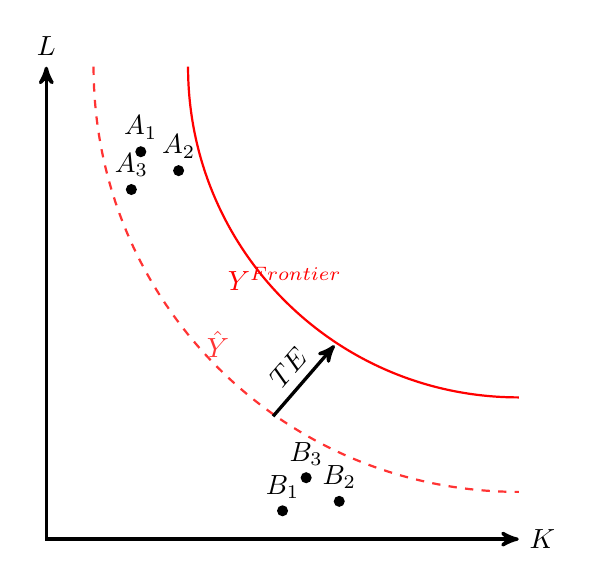
\begin{tikzpicture}[
		scale = 1.2,
		frontier/.style={red,thick},
		axis/.style={very thick , ->, >=stealth', line join=miter},
		region/.style={circle, fill=black, minimum size=4pt, inner sep=0pt, outer sep=-1pt},
		]

	\draw[axis,<->] (5,0) node(xline)[right] {$K$} - | 
				(0,5) node(yline)[above]{$L$};
	\draw[frontier] (1.5,5) to[out=270,in=180] node[above]  {$Y^{Frontier}$} (5,1.5) ;
	\node (A1) [region,label=above:$A_1$] at (1,4.1) {};
	\node (A2) [region,label=above:$A_2$] at (1.4,3.9) {};
	\node (A3) [region,label=above:$A_3$] at (0.9,3.7) {};
	\draw[frontier, red!80, dashed] (0.5,5) to[out=270,in=180] node[above]  {$\hat{Y}$} (5,0.5);
	\node (B1) [region,label=above:$B_1$] at (2.5,0.3) {};
	\node (B2) [region,label=above:$B_2$] at (3.1,0.4) {};
	\node (B3) [region,label=above:$B_3$] at (2.75,0.65) {};
	\draw[->, very thick, black, >=stealth'] (2.4,1.3) -- (3.05,2.05)
		node[sloped, above, midway] {$TE$};
\end{tikzpicture}
\end{center}
\end{frame}

\subsection{Stochastic frontiers}

\begin{frame}{Stochastic frontiers}
\tikzstyle{na} = [baseline=-.5ex]
In general, regional production, $Y$, can be modeled as:
%
\begin{equation*}
Y = f(\mathbf{X};\beta^T)TE,
\label{productionfrontier}
\end{equation*}
%
Assume Cobb-Douglas and $TE = \exp(-U)$, then:
%
\begin{equation*}
\ln Y = \ln A + 
            \beta_1 \ln K + \beta_2 \ln L
        -
        \tikz[baseline]{
            \node[fill=red!20, ellipse,anchor=base] (t2)
            {$U $};
        }
        +
        \tikz[baseline]{
            \node[fill=green!20, ellipse,anchor=base] (t3)
            {$V$};
        },
\label{specification}
\end{equation*}
%
Where usually:
\begin{itemize}
	\item $U \sim N^+ \left(0,\sigma^2_U\right)$
	\item $V \sim N \left(0,\sigma^2_V\right)$
\end{itemize}
\end{frame}

\subsection{Skew-normal alternative}

\begin{frame}{The skew-normal distribution}
\begin{itemize}
	\item Alternative specification, skew normal distribution:
%
\begin{equation*}
Z \sim SN(\alpha) = 2\phi(z)\Phi(\alpha z)
\end{equation*}
%
\pause
\item Which has two types of genesis:
\begin{enumerate}
	\item By convolution: $Z = \delta|U| + \sqrt{1-\delta^2}V$
	\item By conditioning: $Z = (V|U<0)$
	\newline
\end{enumerate}
\pause
\item And is closed under affine transformations: 
\begin{itemize}
	\item if $Y = \mathbf{X}\beta + \sigma Z$ then $Y \sim SN(\mathbf{X}\beta,\sigma, \alpha)$
\end{itemize}
\end{itemize}

\end{frame}

\begin{frame}{Varying the shape parameter $\alpha$}
\begin{figure}[h]
	\center
\begin{tikzpicture} 
\begin{axis}[width=9cm]
\addplot[color=blue, dashed]
table[x=x,y=y1] {SkewNormalDensities.txt};
\legend{$\alpha = -4$}
\end{axis}
\end{tikzpicture}
\label{fig:sn1}
\end{figure}
\end{frame}

\begin{frame}{Varying the shape parameter $\alpha$}
\begin{figure}[h]
	\center
\begin{tikzpicture} 
\begin{axis}[width=9cm]
\addplot[color=blue, dashed]
table[x=x,y=y1] {SkewNormalDensities.txt};
\addplot[color=red, dashed]
table[x=x,y=y2] {SkewNormalDensities.txt};
\legend{$\alpha = -4$,$\alpha = -1$}
\end{axis}
\end{tikzpicture}
\label{fig:sn2}
\end{figure}
\end{frame}

\begin{frame}{Varying the shape parameter $\alpha$}
\begin{figure}[h]
	\center
\begin{tikzpicture} 
\begin{axis}[width=9cm]
\addplot[color=blue, dashed]
table[x=x,y=y1] {SkewNormalDensities.txt};
\addplot[color=red, dashed]
table[x=x,y=y2] {SkewNormalDensities.txt};
\addplot[color=black]
table[x=x,y=y3] {SkewNormalDensities.txt};
\legend{$\alpha = -4$,$\alpha = -1$, $\alpha = 0$}
\end{axis}
\end{tikzpicture}
\label{fig:sn3}
\end{figure}
\end{frame}

\begin{frame}{Varying the shape parameter $\alpha$}
\begin{figure}[h]
	\center
\begin{tikzpicture} 
\begin{axis}[width=9cm]
\addplot[color=blue, dashed]
table[x=x,y=y1] {SkewNormalDensities.txt};
\addplot[color=red, dashed]
table[x=x,y=y2] {SkewNormalDensities.txt};
\addplot[color=black]
table[x=x,y=y3] {SkewNormalDensities.txt};
\addplot[color=red]
table[x=x,y=y4] {SkewNormalDensities.txt};
\legend{$\alpha = -4$,$\alpha = -1$, $\alpha = 0$, $\alpha = 1$}
\end{axis}
\end{tikzpicture}
\label{fig:sn4}
\end{figure}
\end{frame}

\begin{frame}{Varying the shape parameter $\alpha$}
\begin{figure}[h]
	\center
\begin{tikzpicture} 
\begin{axis}[width=9cm]
\addplot[color=blue, dashed]
table[x=x,y=y1] {SkewNormalDensities.txt};
\addplot[color=red, dashed]
table[x=x,y=y2] {SkewNormalDensities.txt};
\addplot[color=black]
table[x=x,y=y3] {SkewNormalDensities.txt};
\addplot[color=red]
table[x=x,y=y4] {SkewNormalDensities.txt};
\addplot[color=blue]
table[x=x,y=y5] {SkewNormalDensities.txt};
\legend{$\alpha = -4$,$\alpha = -1$, $\alpha = 0$, $\alpha = 1$, $\alpha = 4$}
\end{axis}
\end{tikzpicture}
\label{fig:sn5}
\end{figure}
\end{frame}

\section{Benchmarking in the presence of networks}

\subsection{Main concept}

\begin{frame}{Production isoquant revisited (I)}
\tikzstyle{background}=[circle, fill=gray!30,inner sep=0.5cm]
\begin{center}
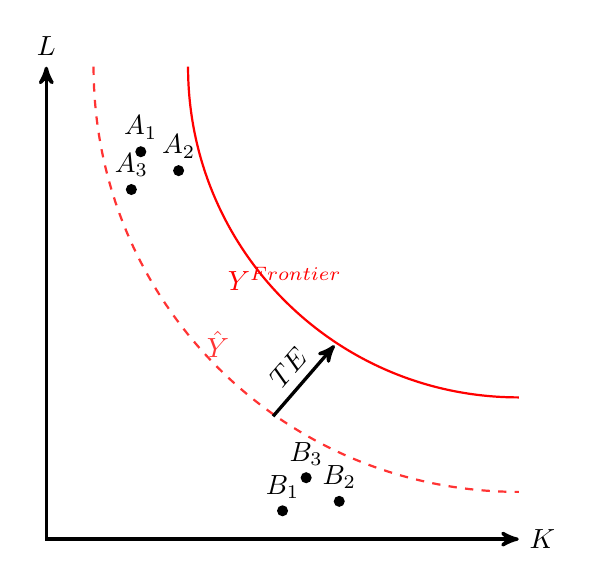
\begin{tikzpicture}[
		scale = 1.2,
		frontier/.style={red,thick},
		axis/.style={very thick , ->, >=stealth', line join=miter},
		region/.style={circle, fill=black, minimum size=4pt, inner sep=0pt, outer sep=-1pt},
		]

	\draw[axis,<->] (5,0) node(xline)[right] {$K$} - | 
				(0,5) node(yline)[above]{$L$};
	\draw[frontier] (1.5,5) to[out=270,in=180] node[above]  {$Y^{Frontier}$} (5,1.5) ;
	\node (A1) [region,label=above:$A_1$] at (1,4.1) {};
	\node (A2) [region,label=above:$A_2$] at (1.4,3.9) {};
	\node (A3) [region,label=above:$A_3$] at (0.9,3.7) {};
	\draw[frontier, red!80, dashed] (0.5,5) to[out=270,in=180] node[above]  {$\hat{Y}$} (5,0.5);
	\node (B1) [region,label=above:$B_1$] at (2.5,0.3) {};
	\node (B2) [region,label=above:$B_2$] at (3.1,0.4) {};
	\node (B3) [region,label=above:$B_3$] at (2.75,0.65) {};
	\draw[->, very thick, black, >=stealth'] (2.4,1.3) -- (3.05,2.05)
		node[sloped, above, midway] {$TE$};
\end{tikzpicture}
\end{center}
\end{frame}

\begin{frame}{Production isoquant revisited (II)}
\tikzstyle{background}=[circle, 
					fill=gray!30,
					inner sep=0.5cm]
\begin{center}
\begin{tikzpicture}[
		scale = 1.2,
		frontier/.style={red,thick},
		axis/.style={very thick , ->, >=stealth', line join=miter},
		region/.style={circle, fill=black, minimum size=4pt, inner sep=0pt, outer sep=-1pt},
		]	
	\draw[axis,<->] (5,0) node(xline)[right] {$K$} - |
				(0,5) node(yline)[above]{$L$};
	\draw[frontier] (1.5,5) to[out=270,in=180] node[above]  {$Y^{Frontier}$} (5,1.5) ;
	\node (A11) [region,label=above:$A_1$] at (1,4.1) {};
	\node (A21) [region,label=above:$A_2$] at (1.4,3.9) {};
	\node (A31) [region,label=above:$A_3$] at (0.9,3.7) {};
	\draw[frontier, red!30, dashed] (0.5,5) to[out=270,in=180] node[above]  {$\hat{Y}$} (5,0.5);
	\draw[frontier, red!80, dashed] (1,5) to[out=270,in=180] node[above]  {$\hat{Y_A}$} (5,0.75);
	\draw[frontier, red!80, dashed] (0.1,5) to[out=270,in=180] node[above]  {$\hat{Y_B}$} (5,0.2);
	\node (B11) [region,label=above:$B_1$] at (2.5,0.3) {};
	\node (B21) [region,label=above:$B_2$] at (3.1,0.4) {};
	\node (B31) [region,label=above:$B_3$] at (2.75,0.65) {};
		\draw[->, very thick, black!30, >=stealth'] (2.4,1.3) -- (3.05,2.05)
		node[sloped, above, midway] {$TE$};
	\draw[->, very thick, black!80, >=stealth'] (1,2.3) -- (2,3.1)
		node[sloped, above, midway] {$TE_B$};
	\draw[->, very thick, black!80, >=stealth'] (3.91,0.89) -- (4.2,1.6)
		node[sloped, above, midway] {$TE_A$};
	\begin{pgfonlayer}{background}
		\node[background, fit =(B11) (B21) (B31), label=left:Country $B$]{};	
		\node[background, fit =(A11) (A21) (A31), label=right:Country $A$]{};	
	\end{pgfonlayer}
\end{tikzpicture}
\end{center}
\end{frame}

\subsection{Spatial frontiers}

\begin{frame}{Introducing a spatial lag (SAR)}
\begin{block}{Because multivariate \emph{skew-normal} distributions are closed under affine transformations, we may write:}
\begin{equation*}
\mathbf{B}\ln(Y) = \ln A + \beta_1 \ln K + \beta_2 \ln L+ Z
\label{spatialfrontier}
\end{equation*}
where $\mathbf{B} = \left(\mathbf{I} - \rho\mathbf{W}\right)$ and with $Z\sim SN (\mathbf{B}^{-1}\mathbf{X}\beta, \Omega, \alpha)$ a multivariate skew normal distribution with $\Omega = \sigma^2 (\mathbf{B} '\mathbf{B})^{-1}$. 
\end{block}
\pause
\begin{block}{Traditional approach}
Other genesis: $\ln Y =\mathbf{B}^{-1} \left( \ln A + \beta_1 \ln K + \beta_2 \ln L+ V\right) - U$, were:
\begin{equation*}
\begin{pmatrix} U \\ V \end{pmatrix} \sim N_{1+k}\left(0,\Omega^\ast\right), \qquad \Omega^\ast=\begin{pmatrix} 1 & -\delta' \\ -\delta & \Omega \end{pmatrix}
\end{equation*}
\end{block}
\end{frame}

\begin{frame}{Introducing a spatial error (SEM)}
\begin{block}{Similar to spatial lag model}
\begin{equation*}
\ln(Y) = \ln A + \beta_1 \ln K + \beta_2 \ln L+ \mathbf{A}^{-1}Z
\label{spatialfrontier}
\end{equation*}
where $\mathbf{A} = \left(\mathbf{I} - \lambda\mathbf{W}\right)$ and with $Z\sim SN (\mathbf{X}\beta, \Omega, \alpha)$ a multivariate skew normal distribution with $\Omega = \sigma^2 (\mathbf{A} '\mathbf{A})^{-1}$. 
\end{block}
\end{frame}

\section{European regional efficiency}

\subsection{Data}

\begin{frame}{Regional production function data}
\begin{itemize}
	\item Cambridge Econometrics Dataset for Employment
	\item Regional value added and capital stock from regional supply and use framework (Thissen et al. 20013a, 2013b and 2013c) 
	\begin{itemize}
			\item Regional trade database between 256 European Nuts2 regions over 15 sectors (2000--2010)
			\item No Perpetual Inventory Method but value added for capital $\rightarrow$ Using country specific interest rates we can then find capital stock ($VA^{capital} = rK$)
	\end{itemize}
	\item Sample period: mean over 2000--2010
	\item Spatial weights matrix $\mathbf{W}$: 4 nearest neighbours
\end{itemize}
\end{frame}

\subsection{Results}

\begin{frame}{Results for energy and manufacturing sector}
\begin{tiny}
\center
\def\onepc{$^{\ast\ast}$} \def\fivepc{$^{\ast}$}
\def\tenpc{$^{\dag}$}
\def\legend{\multicolumn{8}{l}{\footnotesize{Significance levels
:\hspace{1em} $\dag$ : 10\% \hspace{1em}
$\ast$ : 5\% \hspace{1em} $\ast\ast$ : 1\% \normalsize}}}
\centering
\begin{tabular}{l D{.}{.}{3.5}@{} D{.}{.}{2.5}@{} D{.}{.}{2.5}@{} D{.}{.}{2.5}@{} D{.}{.}{2.5}@{} D{.}{.}{2.5}@{} }
\toprule
                  & \multicolumn{1}{c}{OLS} & \multicolumn{1}{c}{SEM} & \multicolumn{1}{c}{SAR} & \multicolumn{1}{c}{Frontier} & \multicolumn{1}{c}{SEM fr.} & \multicolumn{1}{c}{SAR fr.} \\
\midrule
Constant          & 2.40^{***} & 3.16^{***} & 0.46       & 2.50^{***}  & 4.03^{***}  & 0.49       \\
                  & (0.16)     & (0.14)     & (0.26)     & (0.18)      & (0.25)      & (1.22)     \\
$\ln$(Capital)    & 0.77^{***} & 0.58^{***} & 0.70^{***} & 0.76^{***}  & 0.58^{***}  & 0.70^{***} \\
                  & (0.03)     & (0.03)     & (0.03)     & (0.04)      & (0.03)      & (0.03)     \\
$\ln$(Employment) & 0.30^{***} & 0.44^{***} & 0.32^{***} & 0.30^{***}  & 0.44^{***}  & 0.32^{***} \\
                  & (0.03)     & (0.03)     & (0.03)     & (0.04)      & (0.03)      & (0.03)     \\
$\sigma$          & 0.33^{***} & 0.22^{***} & 0.29^{***} & 0.33^{***}  & 0.29^{***}  & 0.29^{*}   \\
                  & (0.01)     & (0.01)     & (0.01)     & (0.02)      & (0.02)      & (0.12)     \\
$\lambda$         &            & 0.79^{***} &            &             & 0.78^{***}  &            \\
                  &            & (0.09)     &            &             & (0.09)      &            \\
$\rho$            &            &            & 0.25^{***} &             &             & 0.25^{***} \\
                  &            &            & (0.03)     &             &             & (0.03)     \\
$\alpha$          &            &            &            & -1.75^{***} & -1.41^{***} & -0.13      \\
                  &            &            &            & (0.53)      & (0.37)      & (5.09)     \\
\midrule
Log Lik.          & -80.10     & 92.28      & 41.45      & 11.03       & 94.86       & 41.45      \\
\bottomrule
\end{tabular}
\end{tiny}
\end{frame}

\begin{frame}{Results all sectors for frontier model with spatial error}
\begin{tiny}
\begin{centering}
\def\onepc{$^{\ast\ast}$} \def\fivepc{$^{\ast}$}
\def\tenpc{$^{\dag}$}
\def\legend{\multicolumn{11}{l}{\footnotesize{Significance levels
:\hspace{1em} $\dag$ : 10\% \hspace{1em}
$\ast$ : 5\% \hspace{1em} $\ast\ast$ : 1\% \normalsize}}}
\centering
\begin{tabular}{l D{.}{.}{2.5}@{} D{.}{.}{2.5}@{} D{.}{.}{2.5}@{} D{.}{.}{3.5}@{} D{.}{.}{3.5}@{} D{.}{.}{3.5}@{} }
\toprule
                  & \multicolumn{1}{c}{Agric.} & \multicolumn{1}{c}{E \& M} & \multicolumn{1}{c}{Constr.} & \multicolumn{1}{c}{Distri.} & \multicolumn{1}{c}{Serv.} & \multicolumn{1}{c}{NM. Serv} \\
\midrule
Constant          & 2.43^{***} & 4.03^{***}  & 2.11^{***}  & 1.24^{***}  & 2.05^{***} & 1.74^{***}  \\
                  & (0.71)     & (0.25)      & (0.22)      & (0.17)      & (0.29)     & (0.19)      \\
$\ln$(Capital)    & 0.68^{***} & 0.58^{***}  & 0.61^{***}  & 0.69^{***}  & 0.71^{***} & 0.61^{***}  \\
                  & (0.03)     & (0.03)      & (0.04)      & (0.03)      & (0.03)     & (0.03)      \\
$\ln$(Employment) & 0.21^{***} & 0.44^{***}  & 0.39^{***}  & 0.30^{***}  & 0.29^{***} & 0.39^{***}  \\
                  & (0.03)     & (0.03)      & (0.04)      & (0.04)      & (0.03)     & (0.04)      \\
$\sigma$          & 0.26^{***} & 0.29^{***}  & 0.28^{***}  & 0.24^{***}  & 0.17^{***} & 0.25^{***}  \\
                  & (0.01)     & (0.02)      & (0.02)      & (0.02)      & (0.01)     & (0.02)      \\
$\alpha$          & -0.03      & -1.41^{***} & -1.19^{***} & -1.54^{***} & -0.02      & -1.68^{***} \\
                  & (1.44)     & (0.37)      & (0.29)      & (0.34)      & (0.75)     & (0.32)      \\
$\lambda$         & 0.57^{***} & 0.78^{***}  & 0.76^{***}  & 0.78^{***}  & 0.59^{***} & 0.81^{***}  \\
                  & (0.08)     & (0.09)      & (0.08)      & (0.08)      & (0.08)     & (0.08)      \\
\midrule
Log Lik.          & 62.92      & 94.86       & 94.19       & 149.78      & 164.88     & 143.52      \\
\bottomrule
\end{tabular}
\end{centering}
\end{tiny}
\end{frame}

\subsection{Regional efficiency}

\begin{frame}{Regional efficiency manufacturing}
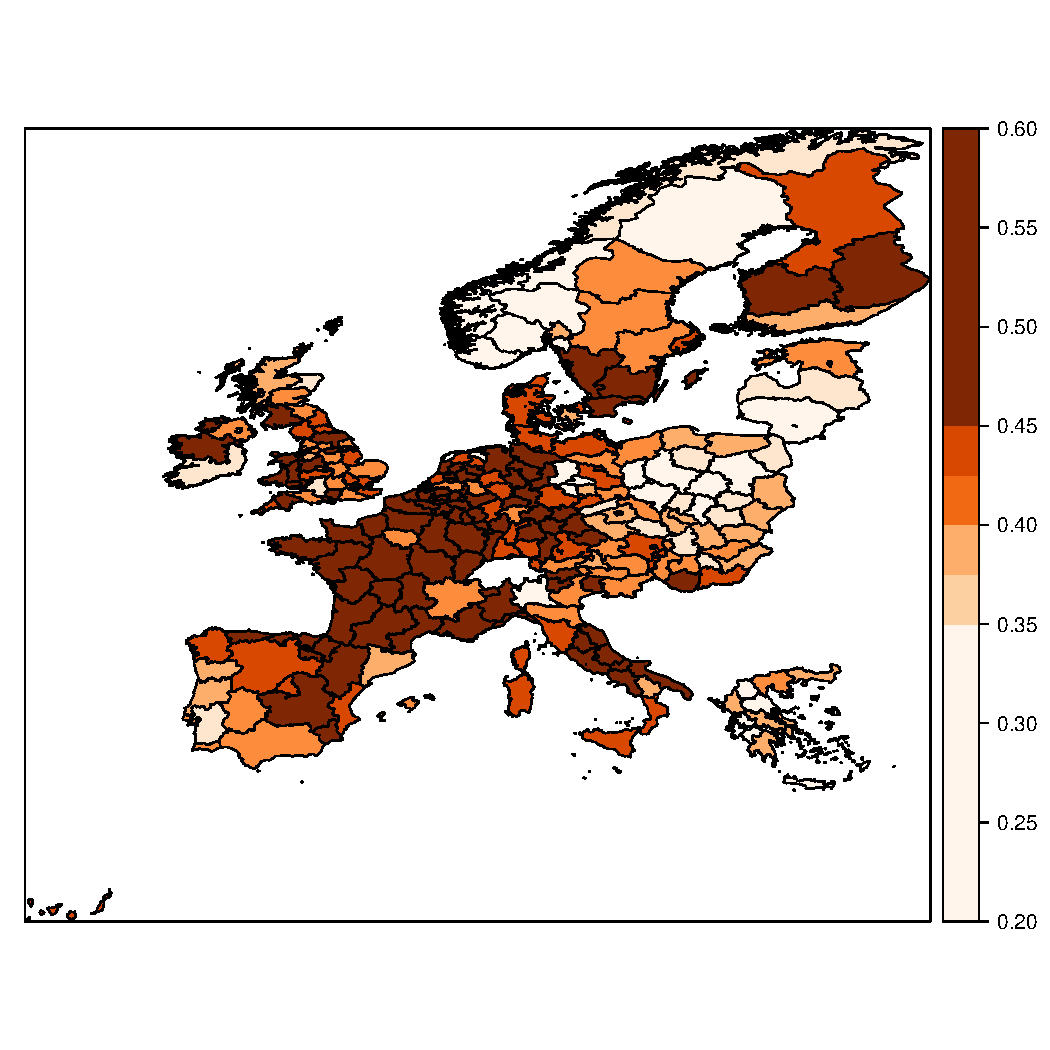
\includegraphics[width=0.8\textwidth]{TEfrontier}
\end{frame}

\begin{frame}{Regional efficiency manufacturing controlling for distance}
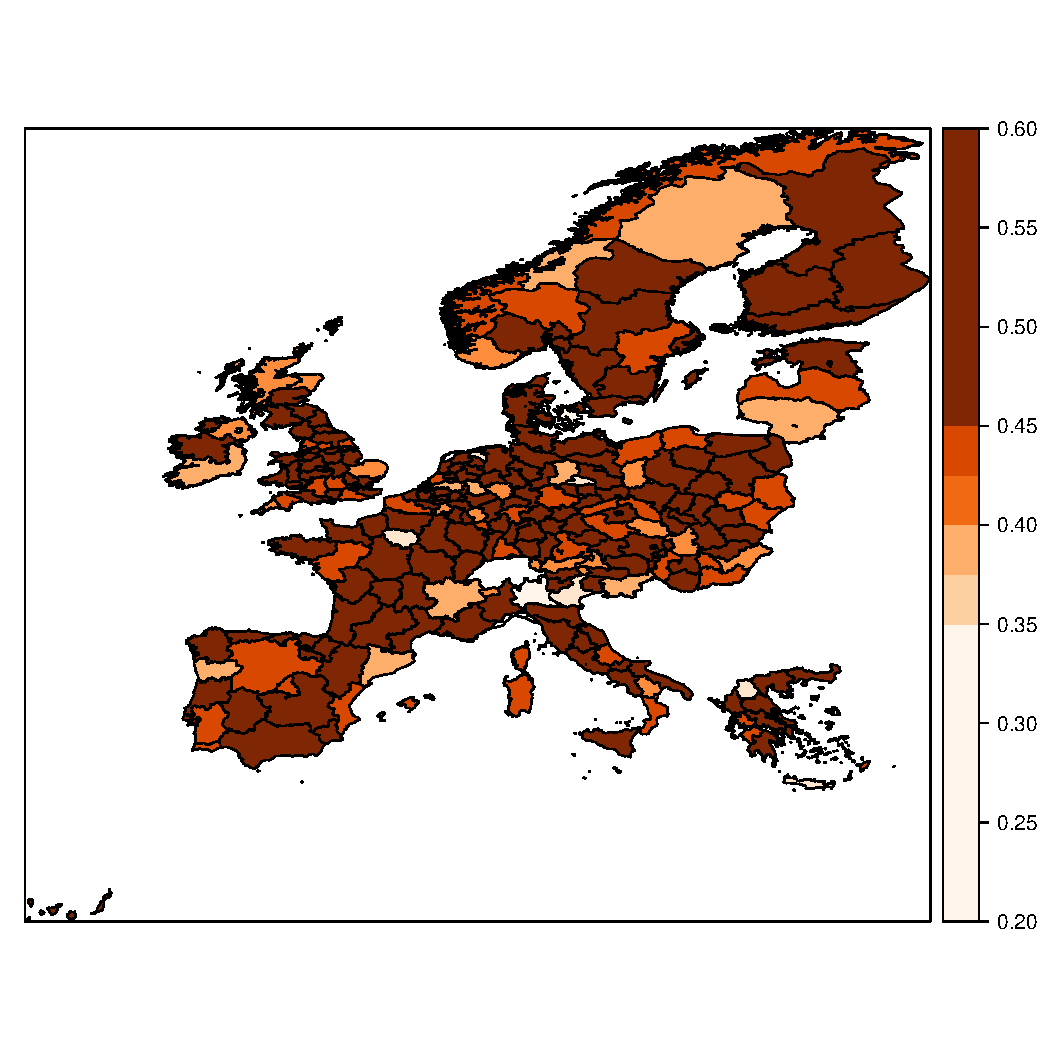
\includegraphics[width=0.8\textwidth]{TEfrontierError}
\end{frame}

\begin{frame}{Difference frontier vs. spatial error frontier for E \& M}
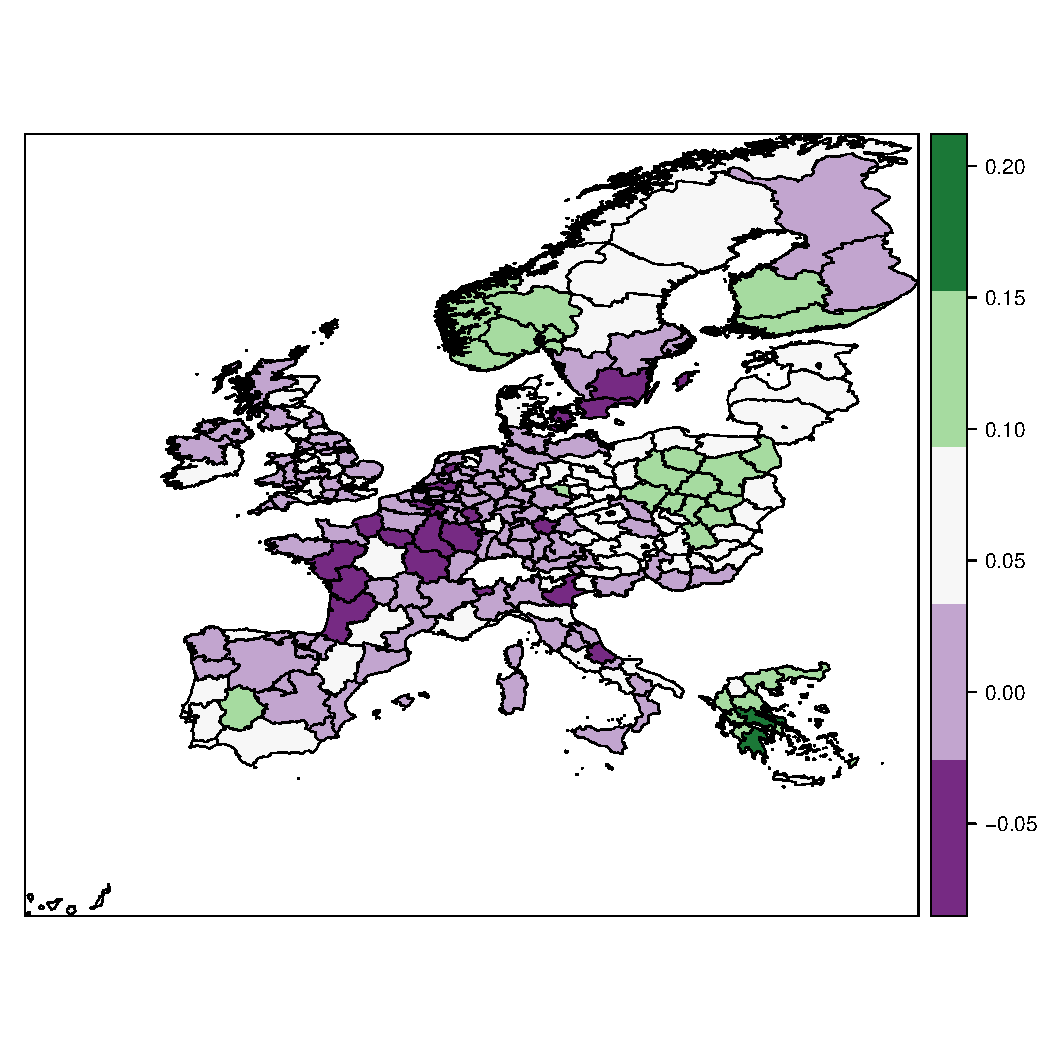
\includegraphics[width=0.8\textwidth]{TEfrontierdiff}
\end{frame}

\begin{frame}{Regional efficiency construction controlling for distance}
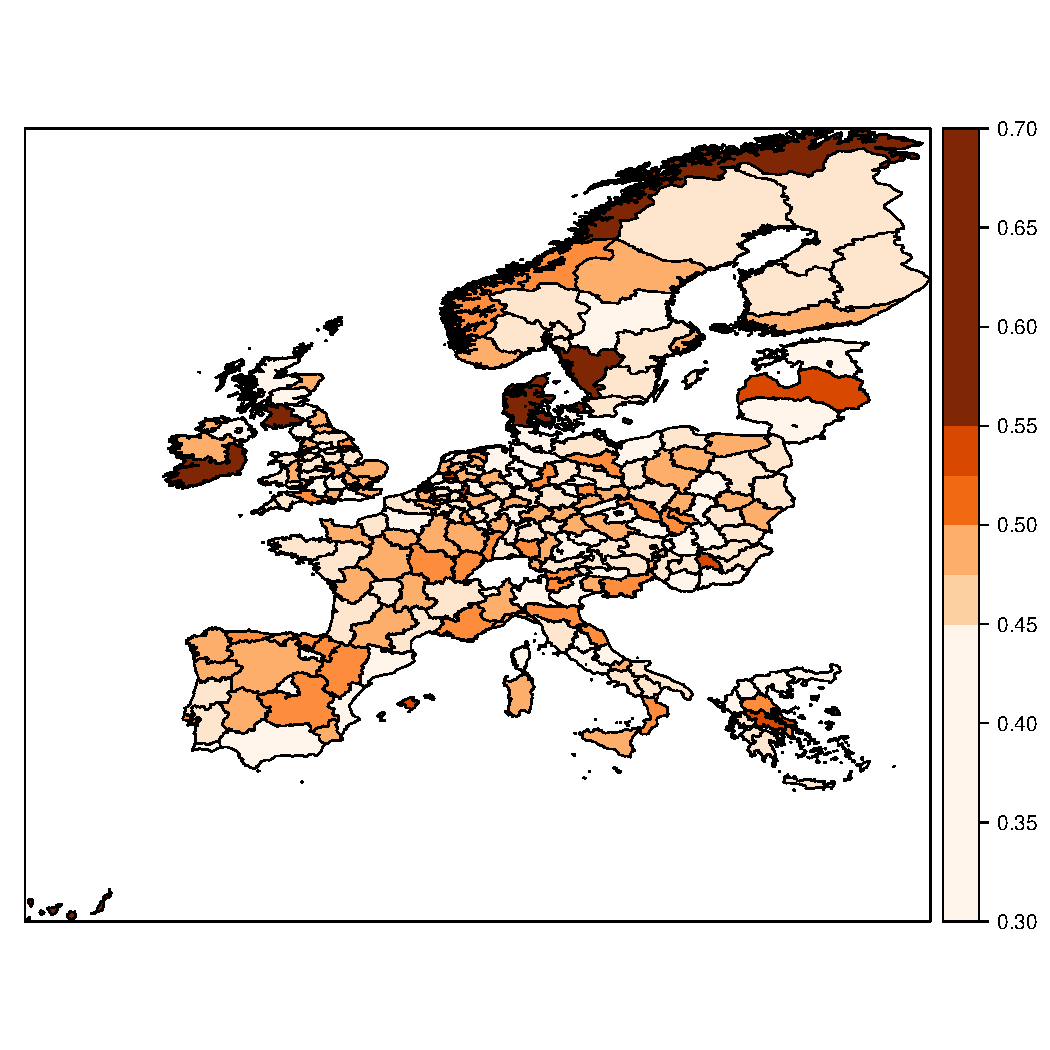
\includegraphics[width=0.8\textwidth]{TEfrontierCon}
\end{frame}

\begin{frame}{Regional efficiency Distribution controlling for distance}
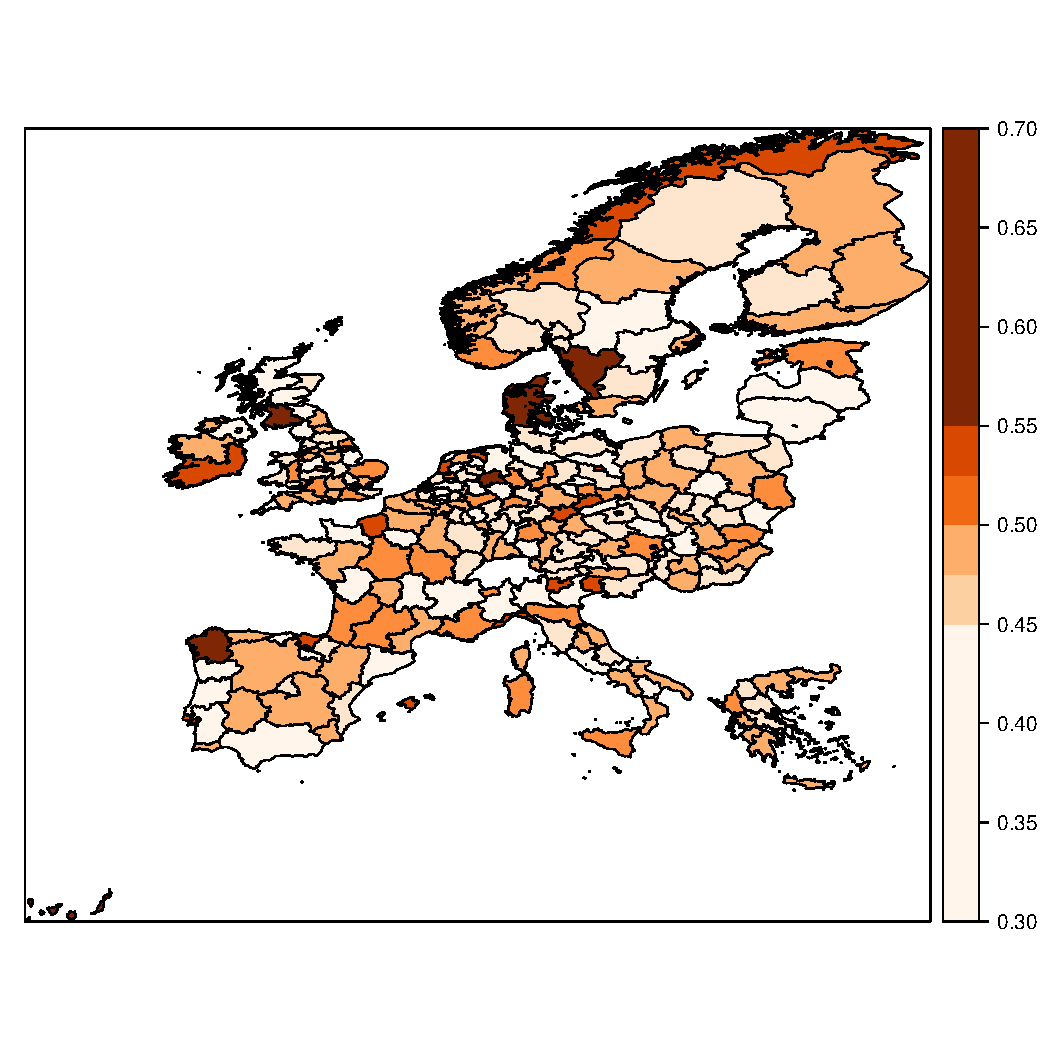
\includegraphics[width=0.8\textwidth]{TEfrontierDist}
\end{frame}

\begin{frame}{Regional efficiency non market services controlling for distance}
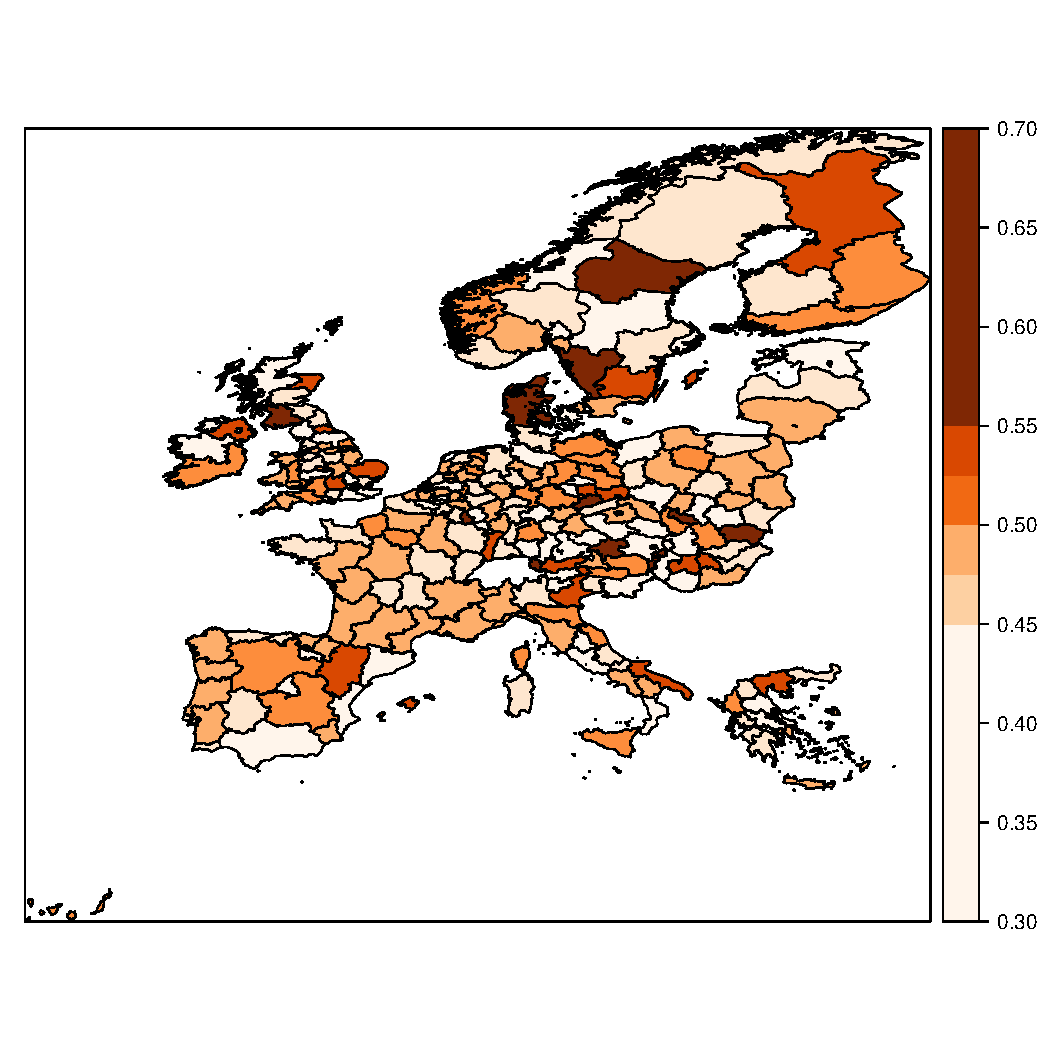
\includegraphics[width=0.8\textwidth]{TEfrontierNMServ}
\end{frame}

\section{In conclusion}

\begin{frame}{Conclusion}
\begin{enumerate}
\item Spatial dependence and stochastic frontiers can be simultaneously and consistently estimated 
\begin{itemize}
	\item relevant for regions and policy
	\item skew-normal distribution is not necessary but much more elegant, more straightforward and less messy
\end{itemize}
\item In the presence of spatial dependence, regional technical inefficiency differences are significantly mitigated
\item Spatial dependence seems to dominate efficiency mechanism, but \ldots
\end{enumerate}
\end{frame}

\begin{frame}{Further research}
\begin{enumerate}
	\item Using panel structure to control for regional fixed effects (first differencing)
	\item Using different weight matrices (FDI, co-patenting and structural trade)
	\item Regional production functions do not always behave as production functions, perhaps due to:
	\begin{itemize}
		\item omitted variables; country dummies
		\item missing human capital
	\end{itemize}
	\item Policy makers might be more interested in what determines (congestion, accessibility, private R\&D) regional efficiency \ldots
\end{enumerate}
\end{frame}

\begin{frame}{Example: spatially varying impact of congestion on efficiency distribution}
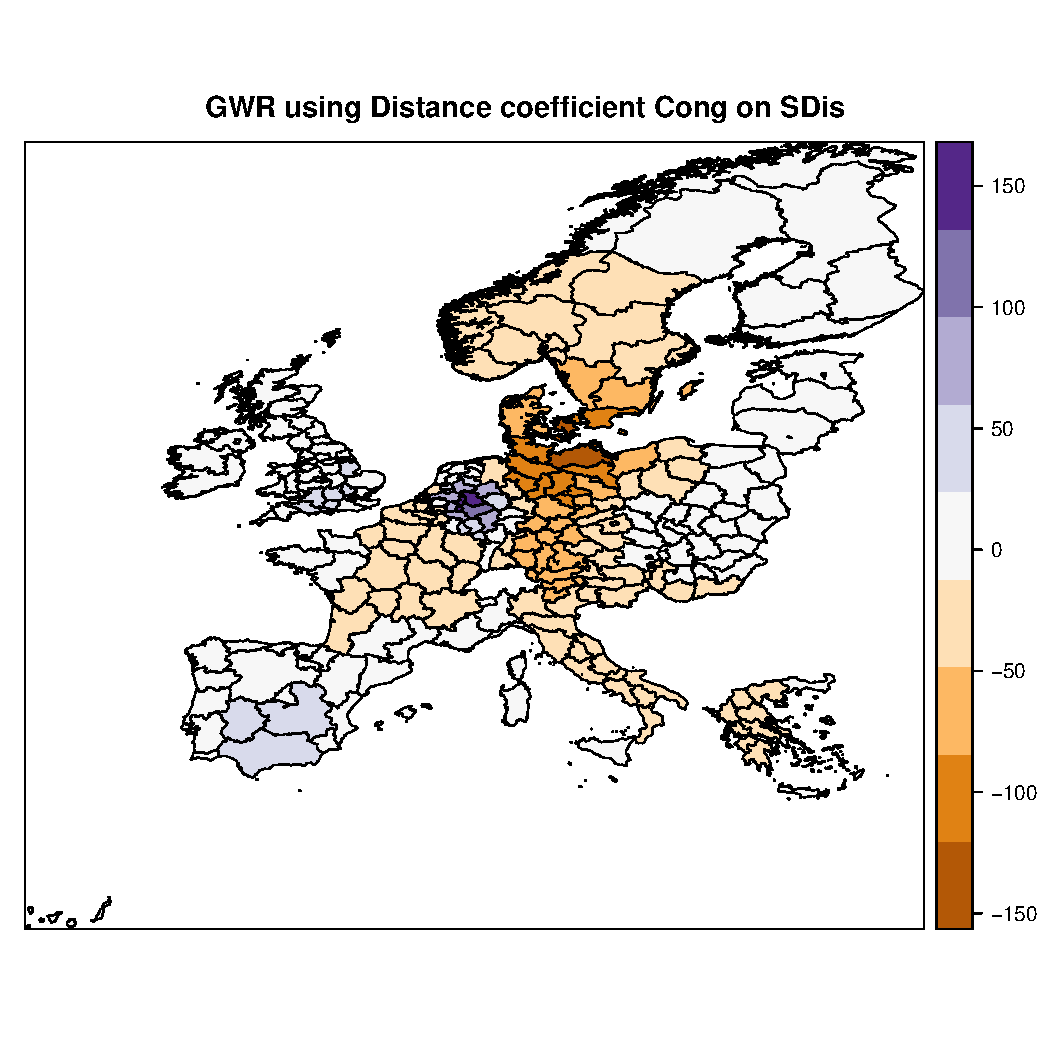
\includegraphics[width=0.8\textwidth]{DistanceSdisCong}
\end{frame}

\end{document}
